% !TeX root = ../thuthesis-example.tex

\chapter{相关工作}


\section{机器学习模型遗忘方法的研究}
这篇文章\cite{yinzhicao2015}最早引入了机器学习遗忘的研究,这篇文章使用统计查询学习的方法对基于贝叶斯方法的机器学习进行了遗忘算法的设计,并没有针对卷积神经网络设计遗忘算法。
这篇文章\cite{antonio2019}对于k-means机器学习的算法设计了遗忘某一类别的方法,可是仍然没有提及卷积神经网络的遗忘算法。
这篇文章\cite{2019arXiv191203817B}提出了一种可以用在神经网络上的遗忘方法。作者将训练数据集分成若干互不相交的部分,然后利用每个部分单独训练出一个神经网络模型,网络最终输出的结果将多个神经网络模型输出的结果综合起来,最终输出一个结果。遗忘的时候,只需要重新训练要遗忘的训练样例所在的神经网络,而无需重新训练所有模型,如图~\ref{fig:machine_unlearning}。这样的方式仍未摆脱重新训练的模式,而且训练如此多的神经网络也造成了参数的浪费。
\begin{figure}
    \centering
    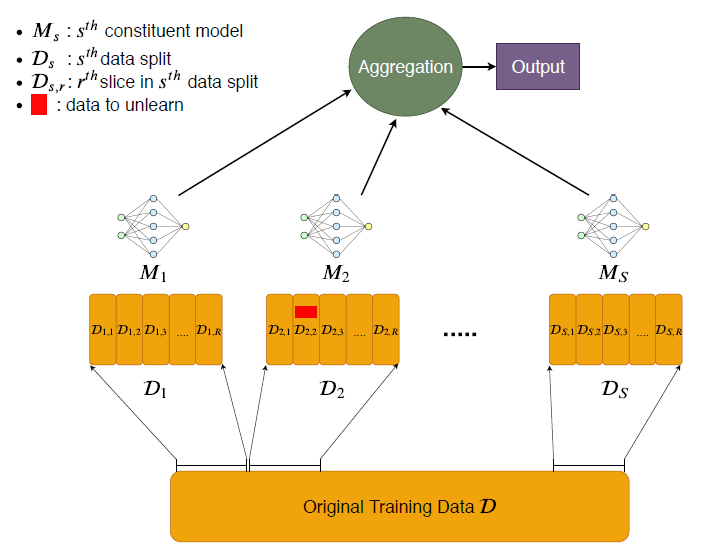
\includegraphics[width=0.9\linewidth]{machine_unlearning.png}
    \caption{将数据集分成若干互不相交集合分别训练}
    \label{fig:machine_unlearning}
\end{figure}
\begin{figure}
    \centering
    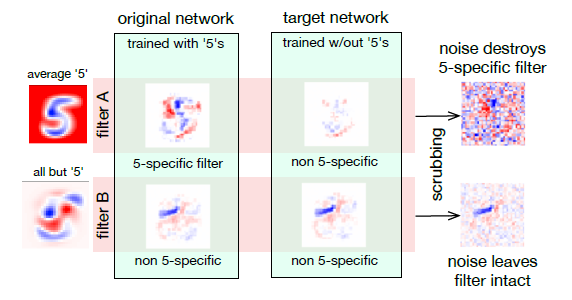
\includegraphics[width=0.9\linewidth]{eternal_sunshine.png}
    \caption{将数据集分成若干互不相交集合分别训练}
    \label{fig:eternal_sunshine}
\end{figure}
这篇文章\cite{Golatkar_2020_CVPR}实现了一种通过在权重上增加噪音的方法来逐渐减少神经网络参数对遗忘数据的信息量,如图~\ref{fig:eternal_sunshine}。同时提出了一些衡量遗忘效果的指标,比如遗忘集的测试准确率,保留集(没有被遗忘的数据集)的测试准确率和测试集的测试准确率。还提出了模型信心的指标,就是对比目标神经网络与此文方法遗忘之后的网络针对遗忘集和保留集输出的交叉熵。这些指标在实际应用上具有参考价值,因此本文也参考了这些评价指标。这篇文章中还提到了一种信息论领域常用到的信息边界的衡量方法,就是计算两个网络模型参数的KL散度距离(Kullback-Leibler Divergence)。这种方法经常用于量化两个随机变量概率分布的相似性。然而,遗忘的目的并不只是简单地让网络的参数去接近目标网络就可以,因此这个衡量指标没有被本文所采用。这个方法虽然在遗忘的效果上达到了较为理想的状态,然而在没有遗忘的类别的准确率上面不是很理想。
这篇文章\cite{Golatkar_2021_CVPR}提出了一种混合训练模型,将训练集分为核心训练集和用户训练集。核心训练集表示学习后不会被遗忘的训练集,用户训练集代表学习后可能会被用户遗忘的训练集。文章中使用了两个神经网络用来训练。第一个网络只用核心训练集进行训练,第二个网络使用第一个网络的输出结果和用户训练集以及核心训练及一起进行训练。当用户申请遗忘数据时,系统会根据没有被遗忘的数据集还有训练好的第一个网络的权重,计算出一个权重变化差,记为$\Delta$w。第二个网络的权重减去这个$\Delta$w即可得到遗忘之后的权重。为了使遗忘的效果更加明显,减去$\Delta$w后再加上一定方差的噪声。文章使用的指标是遗忘集、保留集和测试集的准确率,重新学习时间,激活距离,还有伙伴推断攻击的成功率。激活距离定义为目标遗忘网络和这个方法遗忘后的网络对测试集输出差的第一范数值。伙伴推断攻击的目的是对于给定一个输入,通过一些方法和手段来判断这个输入是否被用于训练网络。其准确率被这篇文章用来当作评价遗忘效果的一个指标。本文借鉴了激活距离和伙伴推断攻击准确率这两个评价指标。
\section{迁移学习的研究}

\section{增强学习的研究}

\section{灾难性遗忘的研究}

\section{本章小结}
